\subsection{Résultats obtenus avec les paramètres initiaux}

\begin{table}[H]
        \centering
        \begin{tabular}{@{}l l l@{}}
            \toprule
            \textbf{Simulation} & Nombre d'épisodes & 400 \\
            & Seuil de mise à jour & 1000 \\
            & Nombre de mise à jour & 20 \\
            & Taille du \emph{mini batch} & 32 \\
            & Nombre de pas par épisode & 200 \\ \midrule
            \textbf{Politique} & Fréquence d'apprentissage & 0,0005\\
            & \(\alpha_{0}\) & 0,01\\
            & Fréquence d'apprentissage de \(\alpha\) & 0,0001\\
            & Entropie ciblée pour \(\alpha\) & -1\\ \midrule
            \textbf{Critique} & Fréquence d'apprentissage & 0,001\\
            & \emph{Discount factor} \(\gamma\) & 0,98\\
            & \(\tau\) & 0,01\\
            \bottomrule
        \end{tabular}
    \caption{Tableaux de la configuration initiale du \emph{Soft Actor Critic}}\label{tab:sac:initial_settings}
\end{table}

Le tableau~\ref{tab:sac:initial_settings} présente les paramètres utilisés pour
les résultats préliminaires présentés ci-dessous.

\begin{figure}[H]
    \centering
    \begin{subfigure}{0.3\textwidth}
        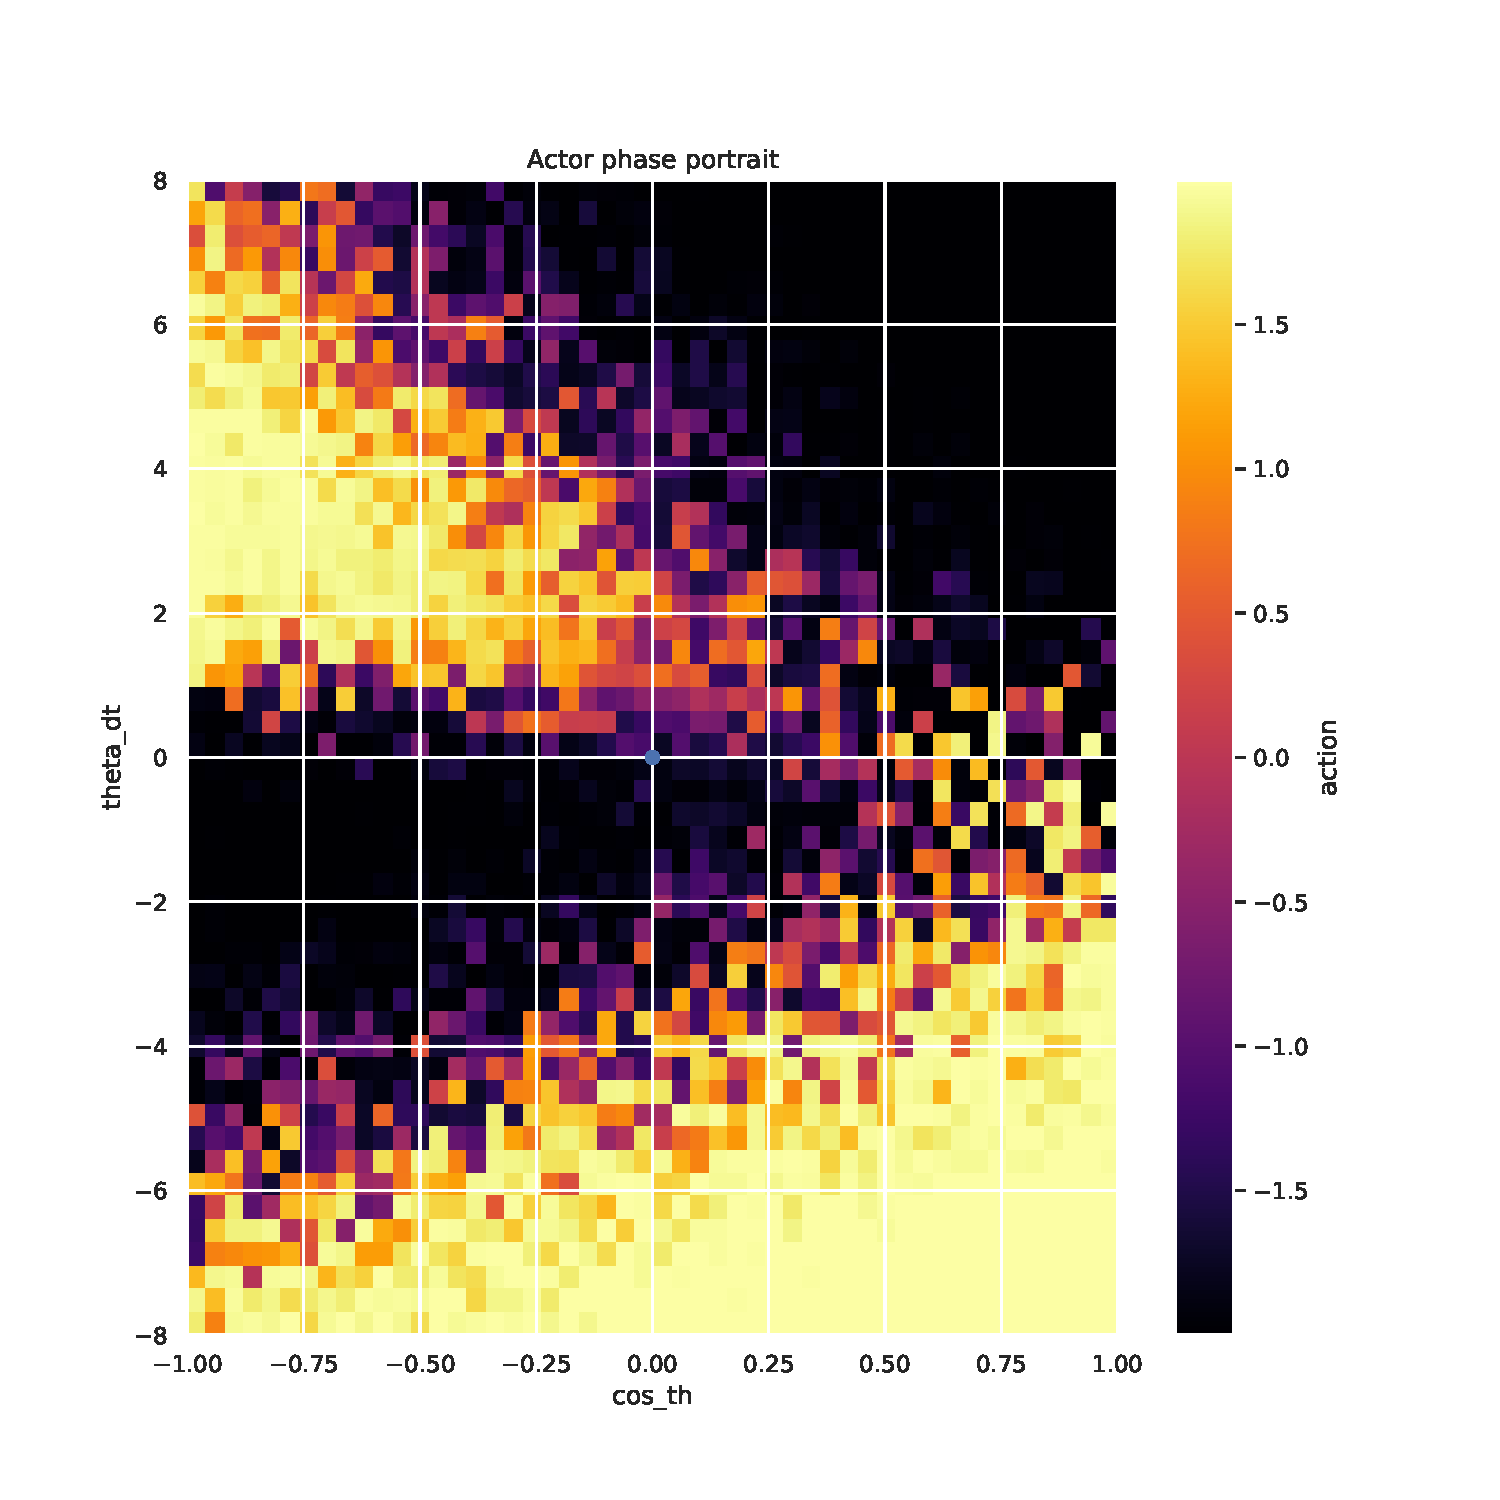
\includegraphics[width=\textwidth]{sac_itr1/1_actor_pg__post_Pendulum-v0.pdf}
        \caption{Acteur entraîné}
    \end{subfigure}
    \begin{subfigure}{0.3\textwidth}
        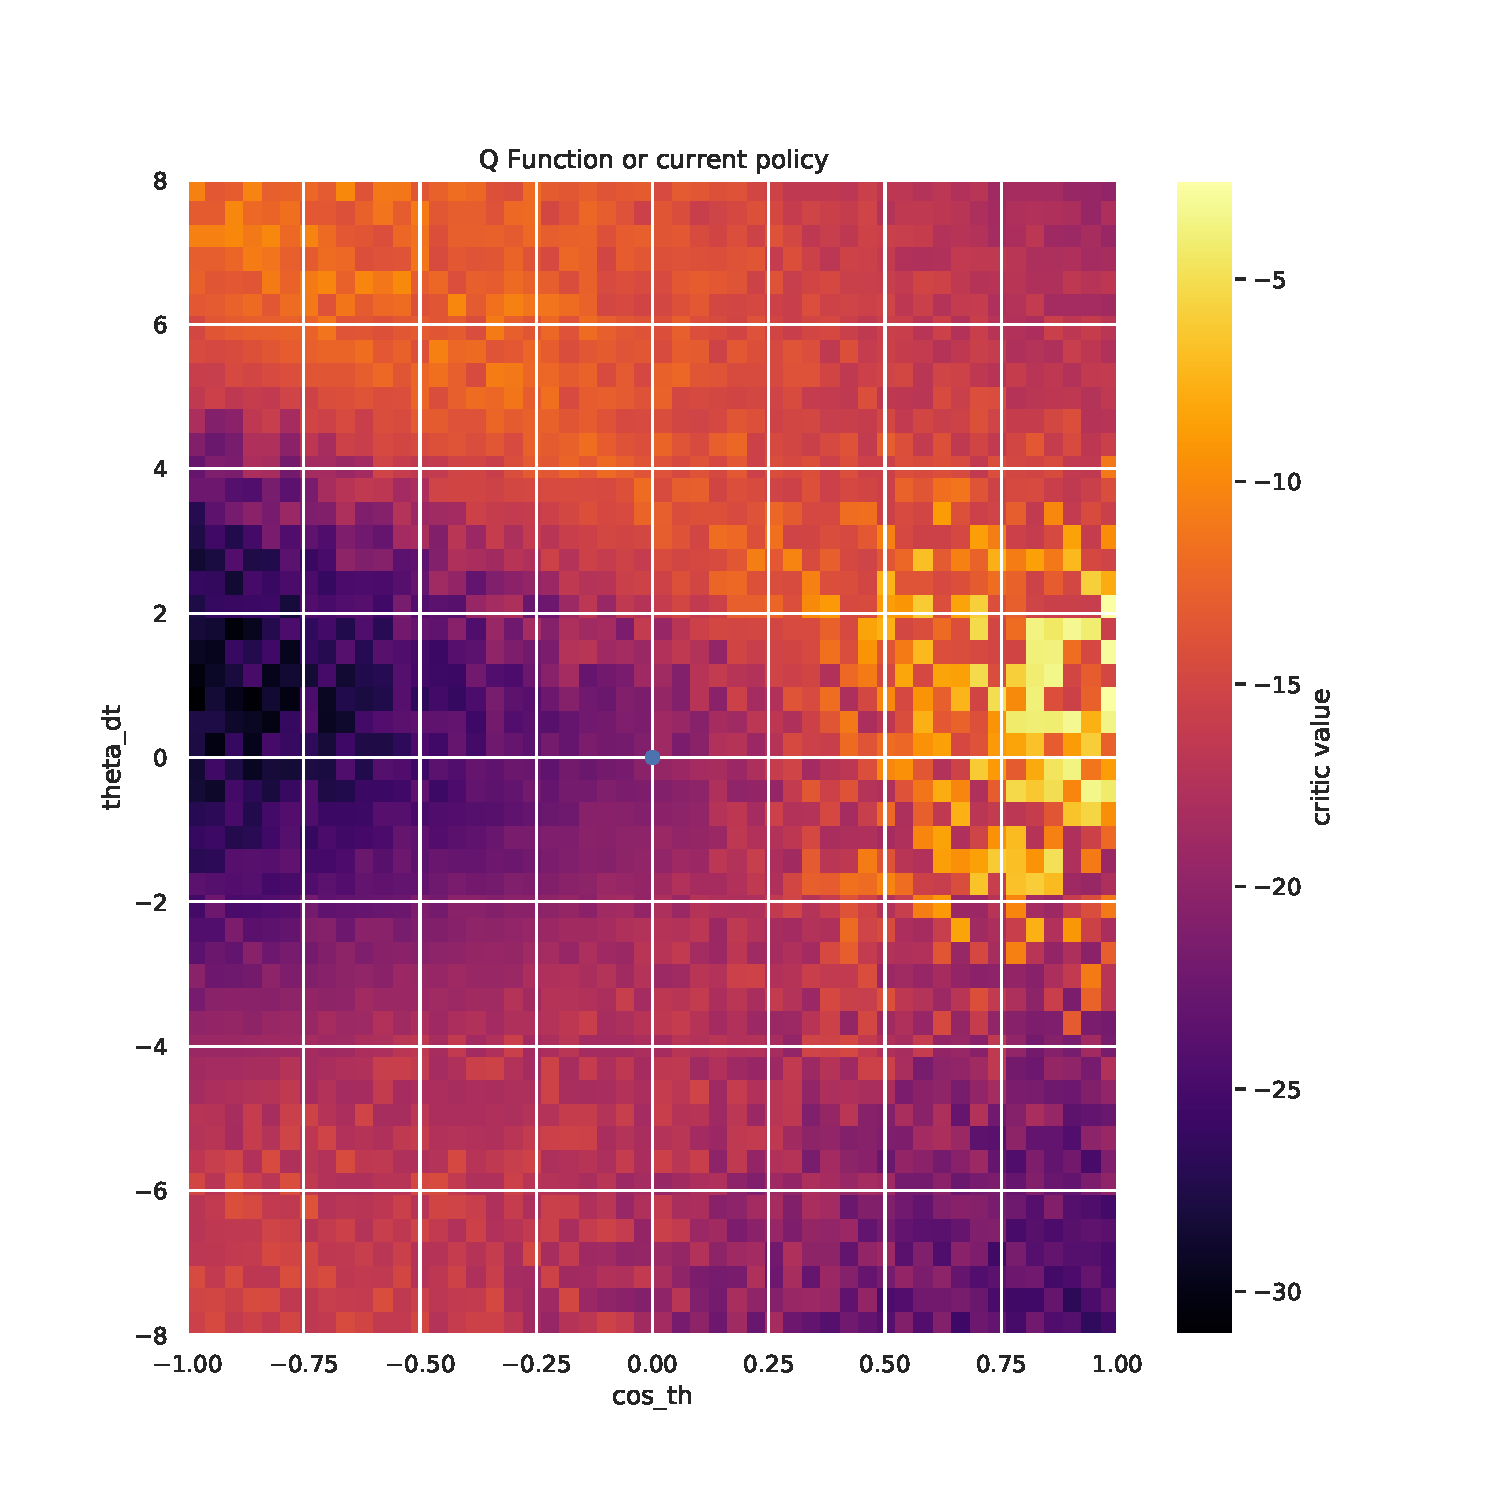
\includegraphics[width=\textwidth]{sac_itr1/1_critic_pg_q1_post_Pendulum-v0.pdf}
        \caption{Critique 1 entraînée}
    \end{subfigure}
    \begin{subfigure}{0.3\textwidth}
        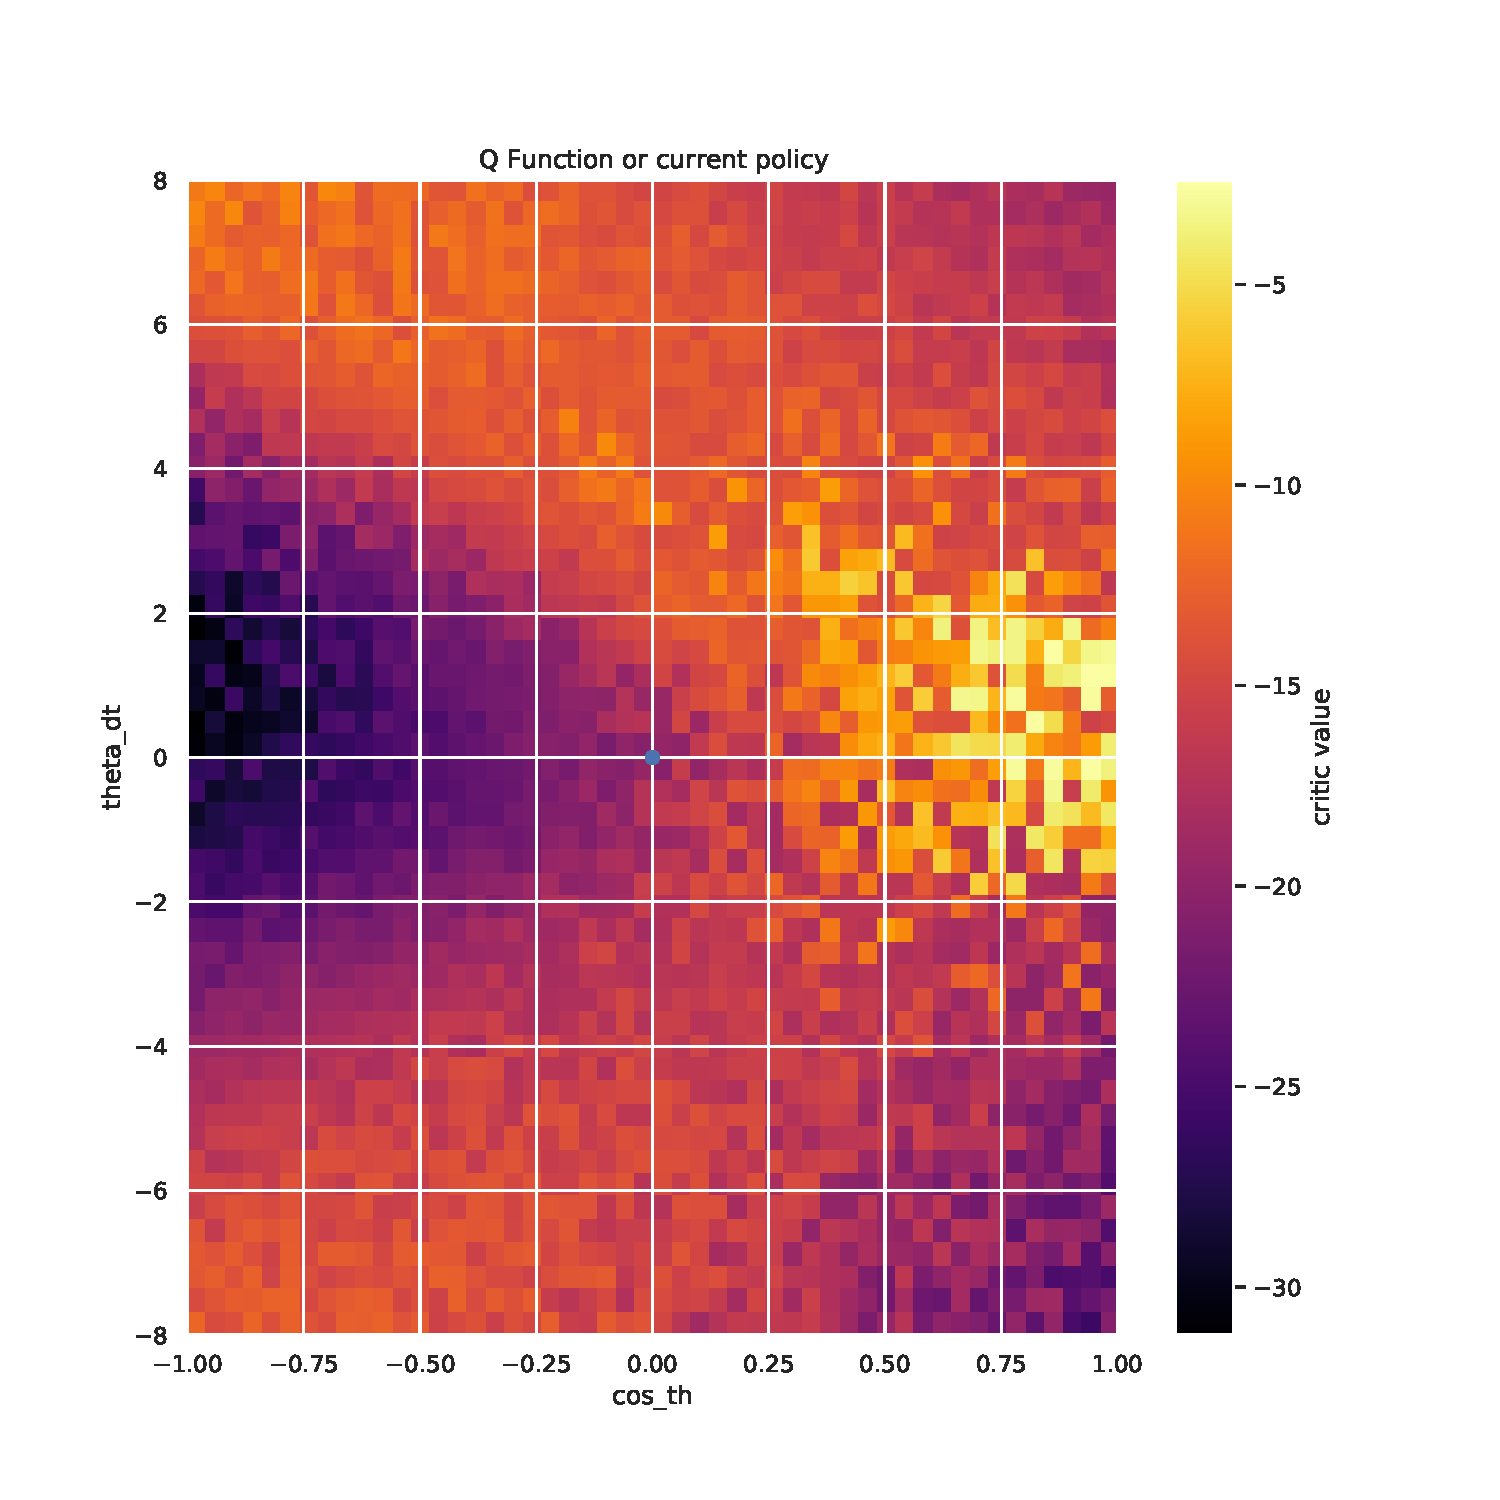
\includegraphics[width=\textwidth]{sac_itr1/1_critic_pg_q2_post_Pendulum-v0.pdf}
        \caption{Critique 2 entraînée}
    \end{subfigure}
    \caption{Valeurs de l'acteur et de la critique avec l'algorithme SAC dans un cas où l'apprentissage est fructueux}\label{fig:sac:preli_success}
\end{figure}

La figure~\ref{fig:sac:preli_success} présente une critique bien entrainée. Par
ailleurs, nous obervons une grande ressemblance dans les deux critiques.

En effet, nous observons que l'acteur cherche à accélérer le pendule lorsqu'il
est en bas en choisissant un couple proportionnel au cosinus de l'angle et à la
vitesse du pendule. À l'inverse, quand le pendule est vers le haut, le couple
est opposé et proportionnel à la vitesse du pendule. Cela à pour effet d'amener
le pendule vers le haut.

Nous observons que la critique a une valeur très négative quand le pendule est
en bas à vitesse nulle ou en haut à vitesse élevé. Ce résultat est attendu
puisqu'il s'agit des états qui conduisent à avoir une plus faible récompense.

\begin{figure}[H]
    \centering
    \begin{subfigure}{0.3\textwidth}
        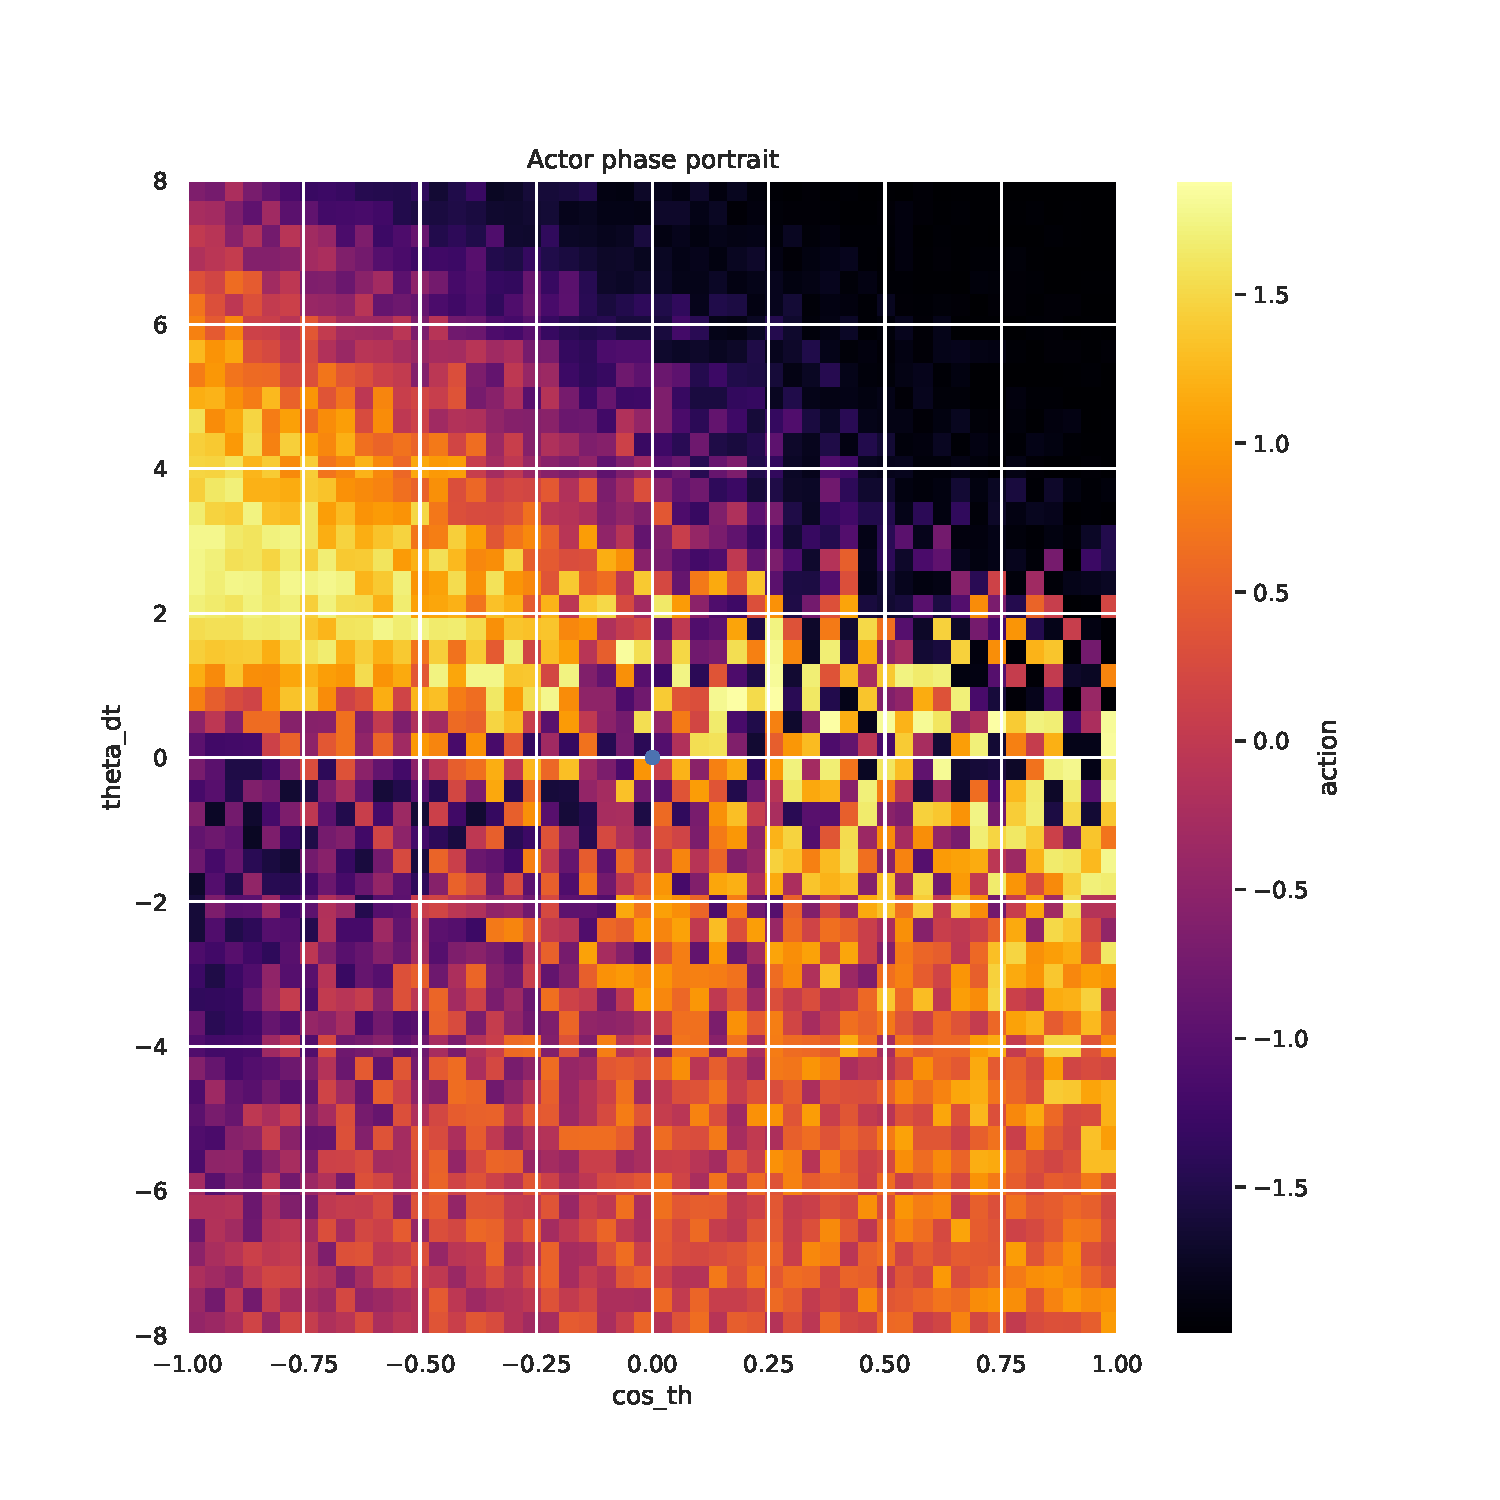
\includegraphics[width=\textwidth]{sac_itr1/6_actor_pg__post_Pendulum-v0.pdf}
        \caption{Acteur entraîné}
    \end{subfigure}
    \begin{subfigure}{0.3\textwidth}
        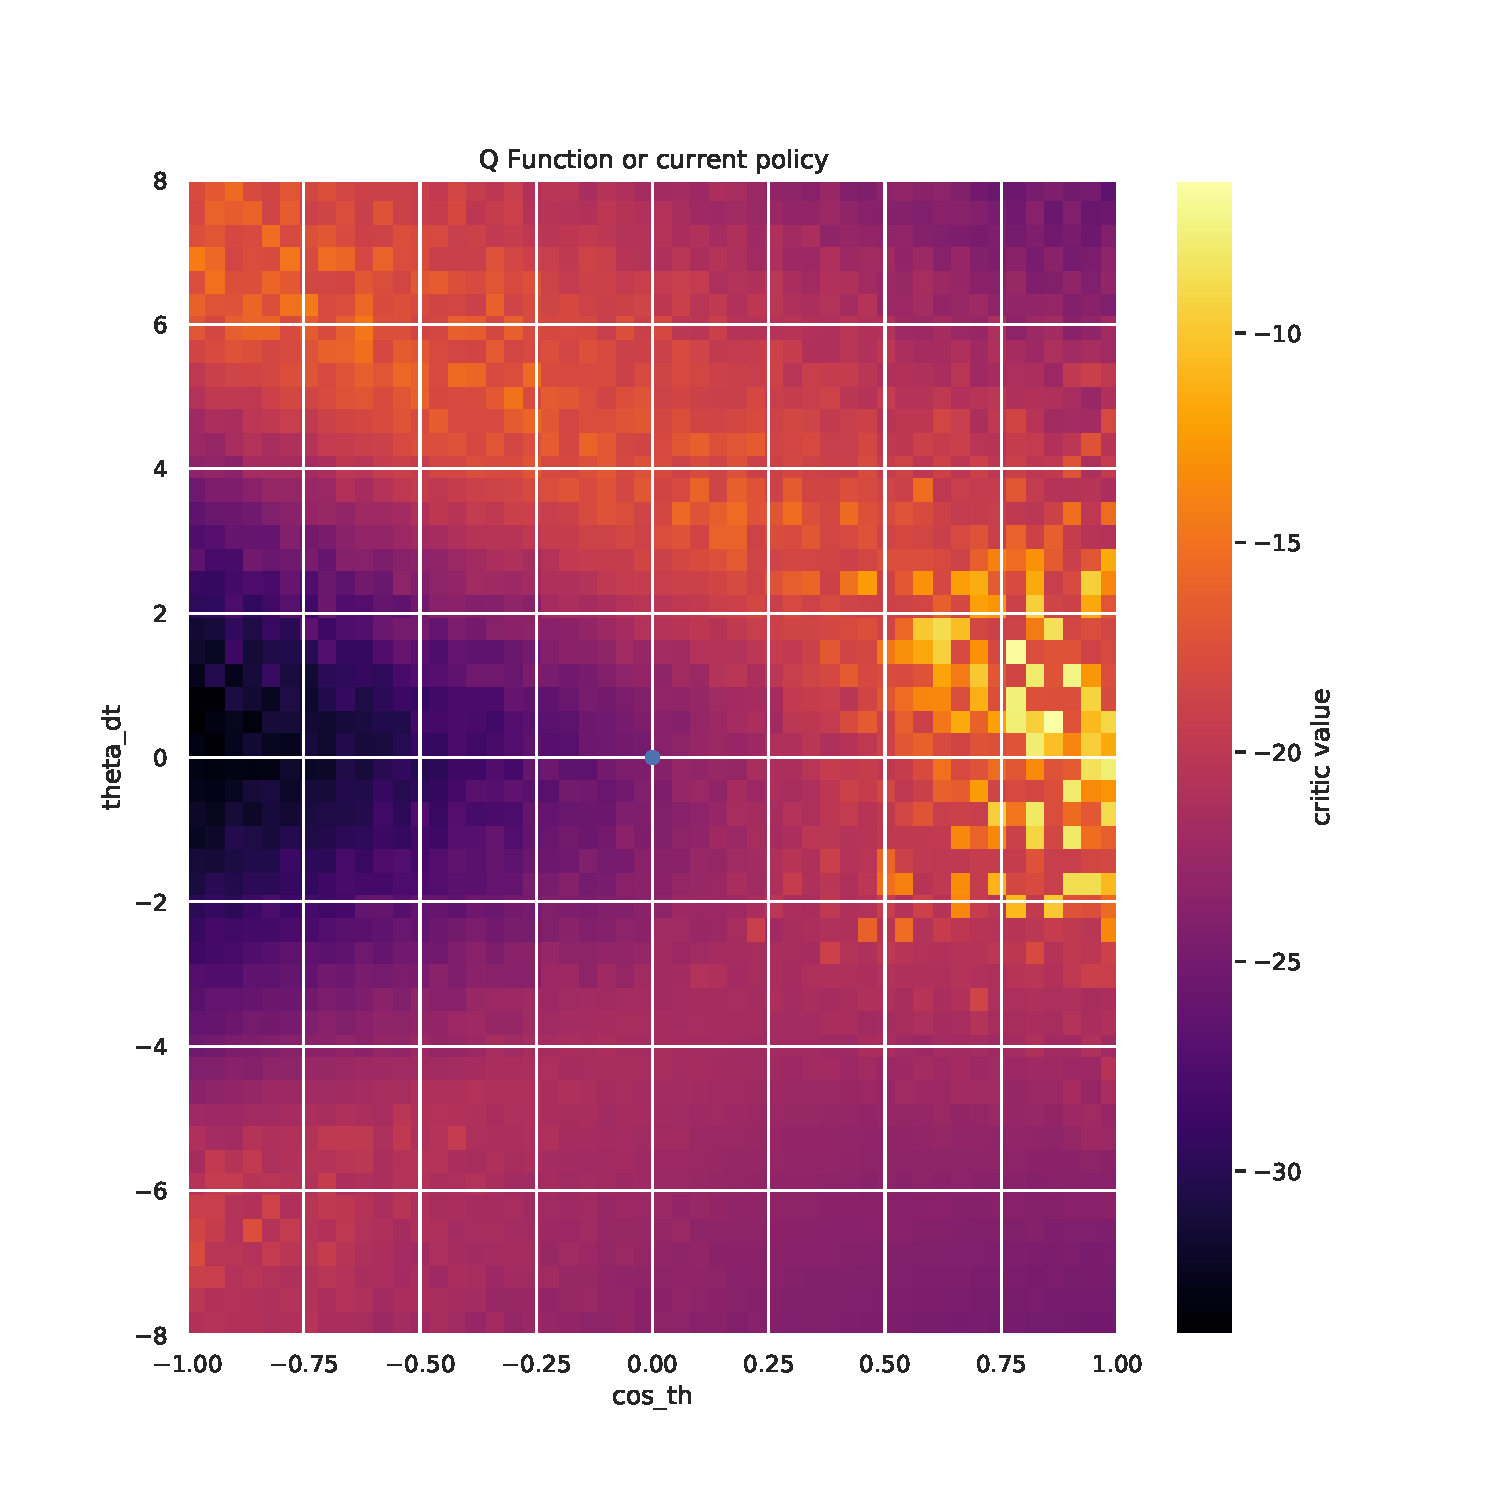
\includegraphics[width=\textwidth]{sac_itr1/6_critic_pg_q1_post_Pendulum-v0.pdf}
        \caption{Critique 1 entraînée}
    \end{subfigure}
    \begin{subfigure}{0.3\textwidth}
        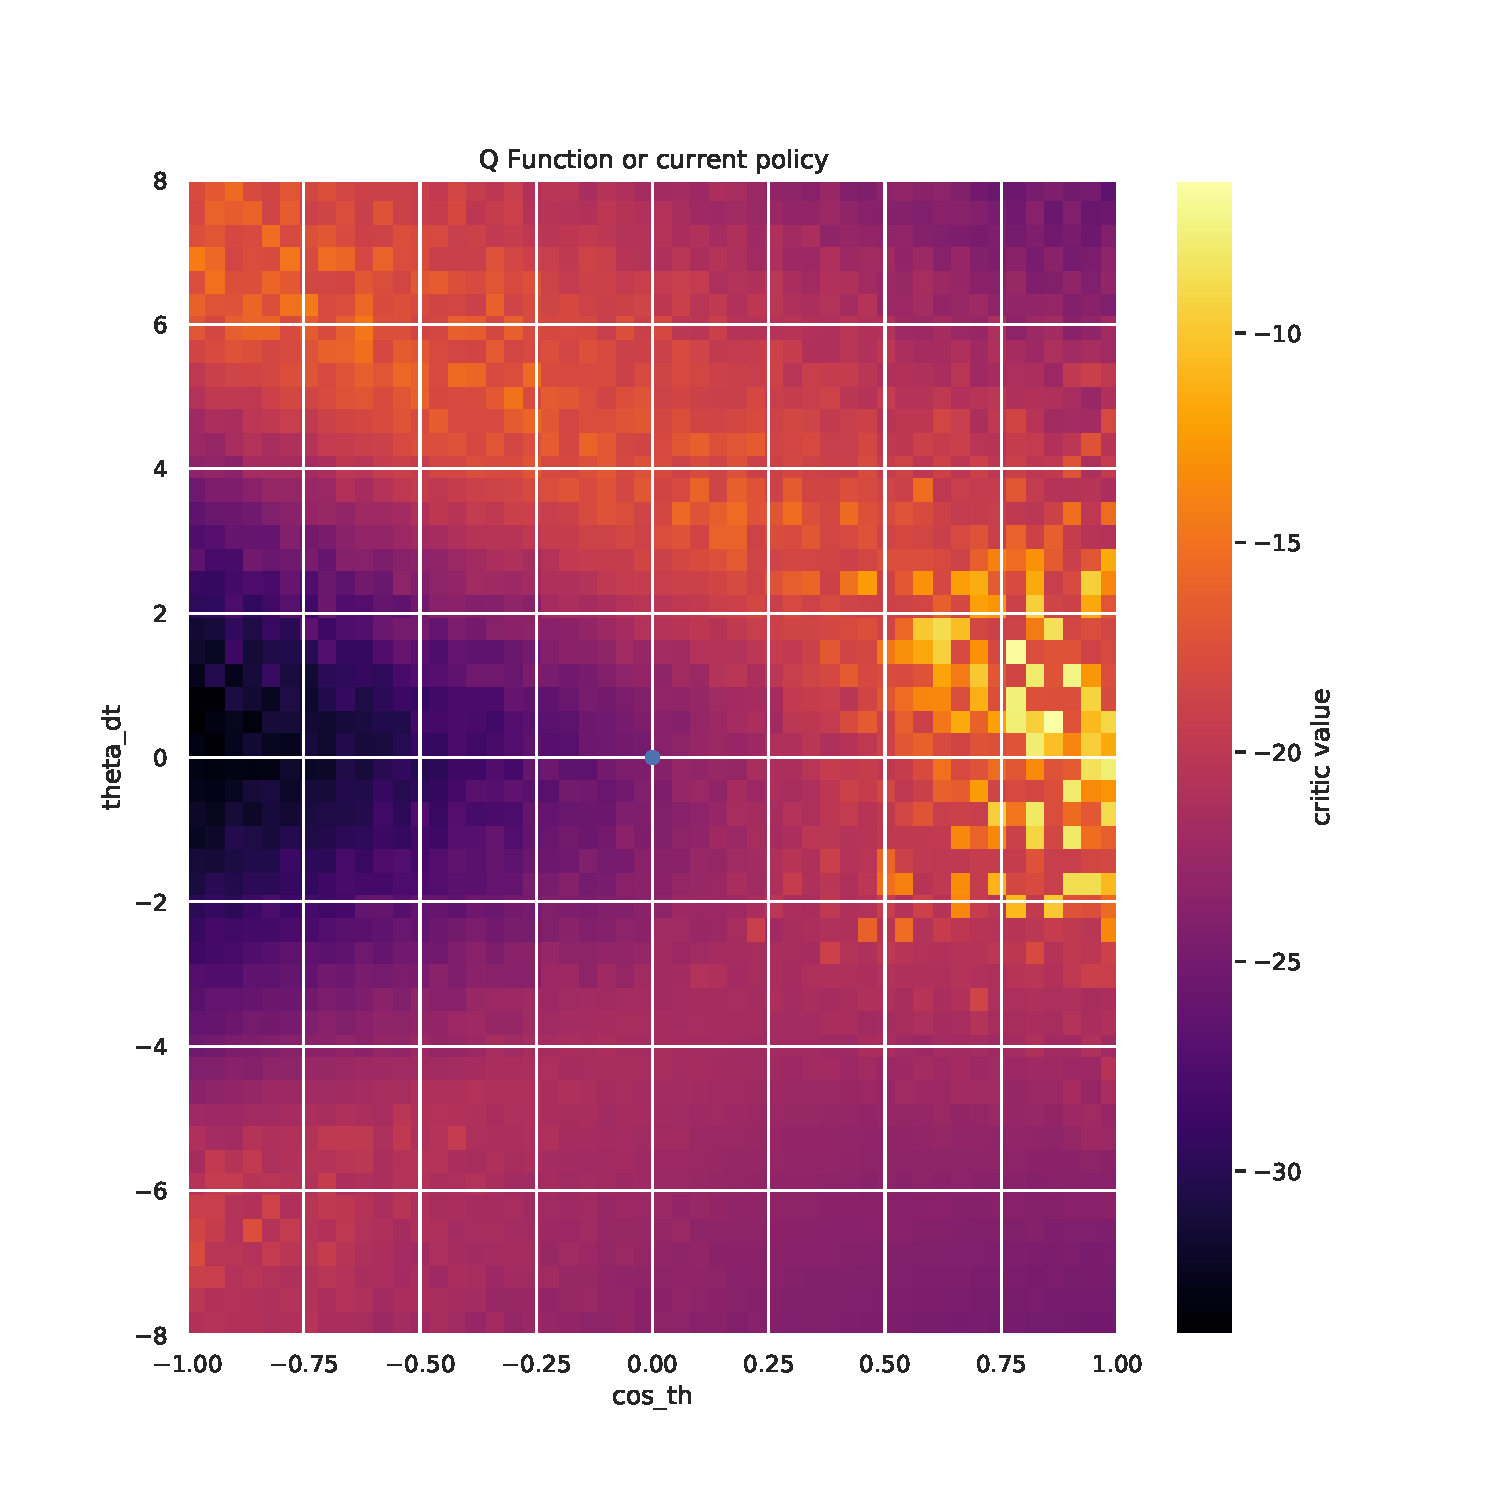
\includegraphics[width=\textwidth]{sac_itr1/6_critic_pg_q1_post_Pendulum-v0.pdf}
        \caption{Critique 2 entraînée}
    \end{subfigure}
    \caption{Valeurs de l'acteur et de la critique avec l'algorithme SAC dans un cas où l'apprentissage n'est pas fructueux}\label{fig:sac:preli_failed}
\end{figure}

La figure~\ref{fig:sac:preli_failed} présente un acteur et une critique mal
entrainée. Au cours de la même exécution. En effet, nous avons répété 10 fois
l'expérience. À toutes les itérations, les deux critiques sont similaires. Nous
n'en présenterons plus qu'une dans la suite de ce document.

Nous observons que les transitions des valeurs sont très dousses
particulièrement quand la vitesse est négative. Cela indique une mauvaise
exploration.

De la même façon, la critique a des variations très dousses qui indique un
mauvais apprentissage.

Ces deux résultats sont communs au cours de nos 10 itérations.

\begin{figure}[H]
    \centering
    \begin{subfigure}{0.30\textwidth}
        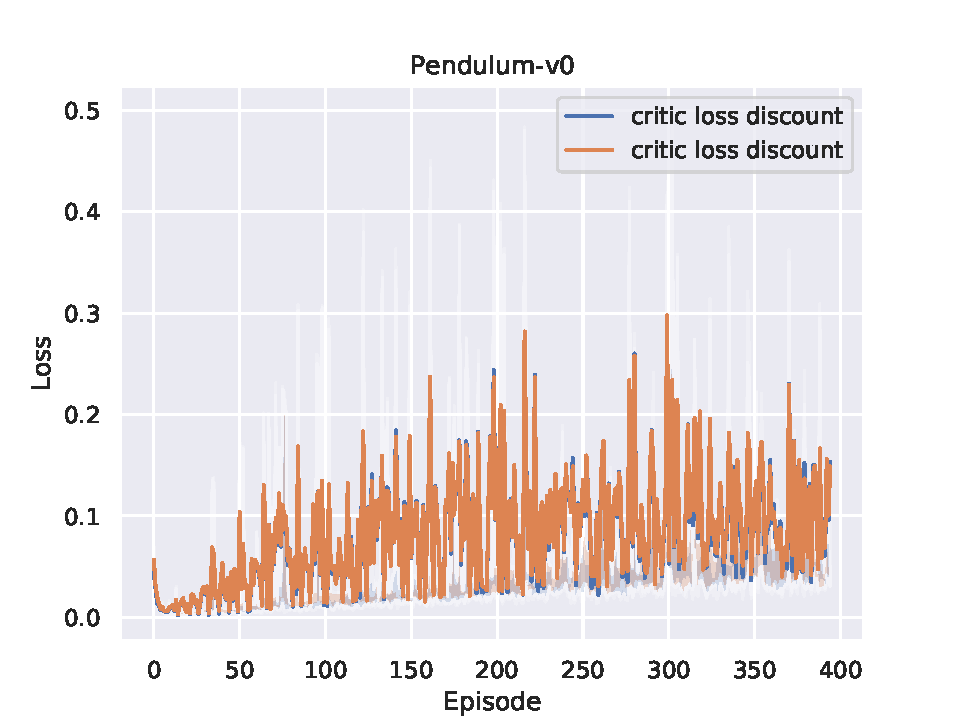
\includegraphics[width=\textwidth]{sac_itr1/critic_loss_Pendulum-v0_pg_dataset_td_trajs_400_update_threshold_1000_nb_updates_20_gamma_0.98_tau_0.01_nstep_5_lr_act_0.0005_lr_critic_0.001_init_alpha_0.01_lr_alpha_0.001_target_entropy_alpha_-1.0pg.pdf}
        \caption{Perte de la critique}
    \end{subfigure}
    \begin{subfigure}{0.30\textwidth}
        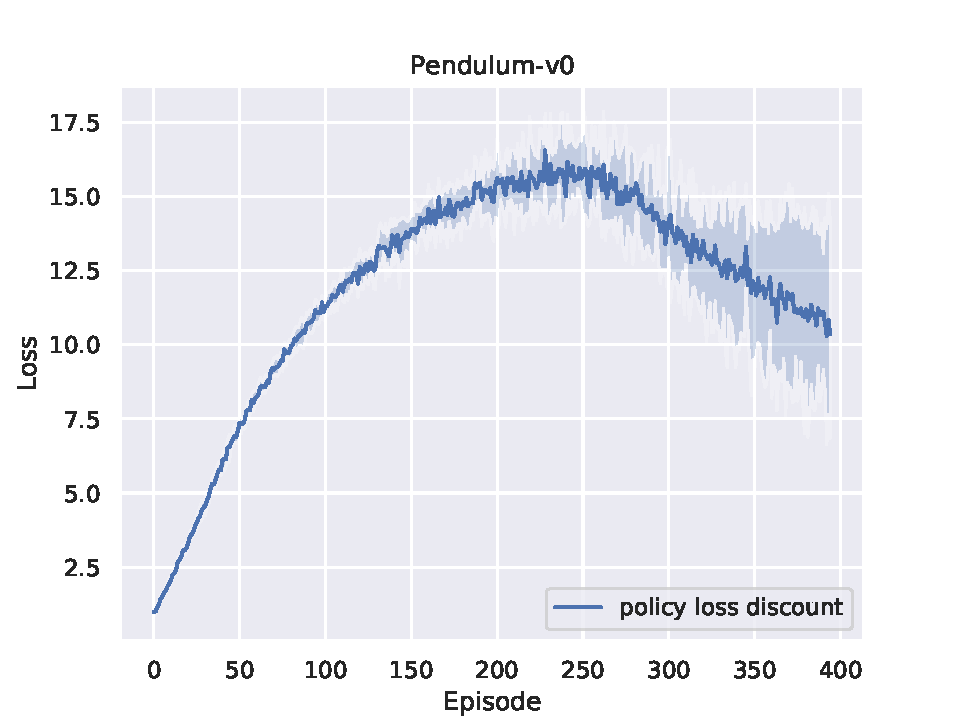
\includegraphics[width=\textwidth]{sac_itr1/policy_loss_Pendulum-v0_pg_dataset_td_trajs_400_update_threshold_1000_nb_updates_20_gamma_0.98_tau_0.01_nstep_5_lr_act_0.0005_lr_critic_0.001_init_alpha_0.01_lr_alpha_0.001_target_entropy_alpha_-1.0pg.pdf}
        \caption{Perte de la politique}
    \end{subfigure}
    \begin{subfigure}{0.30\textwidth}
        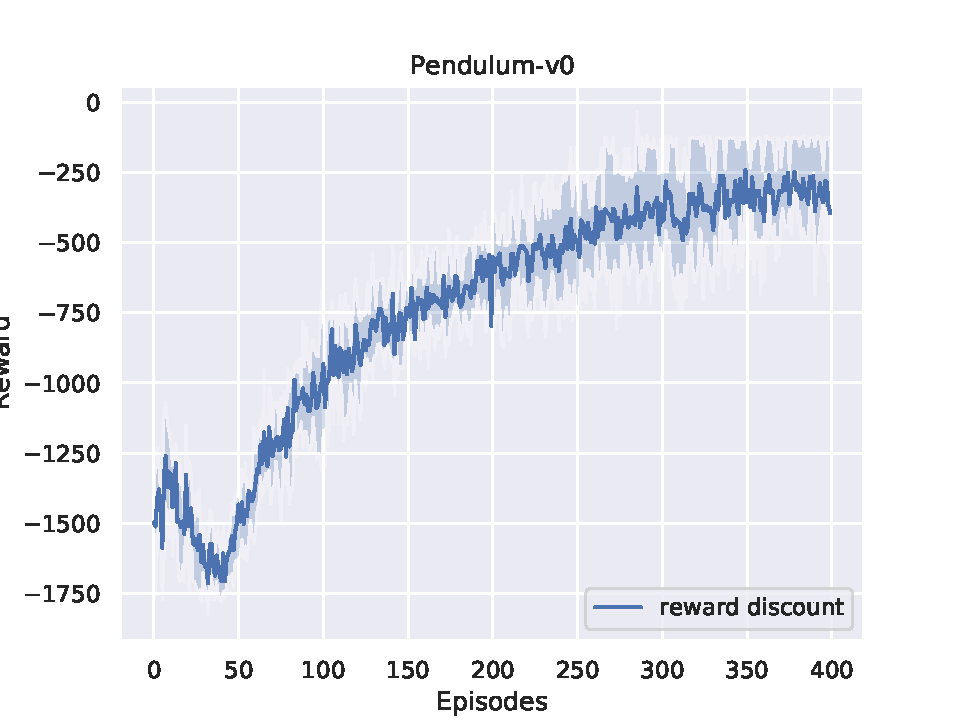
\includegraphics[width=\textwidth]{sac_itr1/rewards_Pendulum-v0_pg_dataset_td_trajs_400_update_threshold_1000_nb_updates_20_gamma_0.98_tau_0.01_nstep_5_lr_act_0.0005_lr_critic_0.001_init_alpha_0.01_lr_alpha_0.001_target_entropy_alpha_-1.0.pdf}
        \caption{Récompense au cours des épisodes}
    \end{subfigure}
    \caption{Résultats obtenus par 10 répétitions avec les paramètres initiaux}\label{fig:sac:results}
\end{figure}

D'après la figure~\ref{fig:sac:results}, la perte de la critique est très bruité
néanmoins, les valeurs sont croissantes, mais reste très faibles. Donc
l'apprentissage de la critique se déroule bien.

La perte de la politique croit initialement. Ce comportement est tout à fait
attendu au début de l'apprentissage. Ensuite, la perte diminue ce qui indique
que la politique s'améliore et réalise la meilleure action selon elle.
Cependant, nous observons que cette phase de décroissance est très variantes
d'une itération à l'autre.

La récompense croit au fil des épisodes donc l'apprentissage conduit à une
amélioration de la politique. Aux environs des 400 épisodes, la pente est très
faible, ce qui nous laisse penser que l'apprentissage est presque terminé.

Nous observons en cours d'apprentissage que le coefficient \(\alpha\) décroit
initialement puis croit jusqu'à valoir environ 0,02 dans les itérations où la
récompense est maximale.

Nous décidons de définir \(\alpha_{0}=0,02\). Nous pensons obtenir plus de
politiques qui convergent vers une récompense plus élevée. Par conséquent, nous
pensons observer une décroissance de la perte de la politique plus importante.
